\chapter{Results and Discussion}
\label{chapter:Results and Discussion}

\section{Results and Discussion}
In this chapter, we evaluate the proposed algorithm using real data acquire using 
the camera rig system illustrated in \ref{ fig:rigsetup} and 
approaches \todo{ define approaches}

\section{Datasets}

\subsection{Part based model}
We define, as describe in chapter \ref{chapter:Implementation}, a full-body skeleton 
for the fish annotated dataset, with this information we construct a fully supervised 
dataset, from which we learn a flexible mixture of parts, We show the full-body model learned
from the created data set, for 3, 5, 7, 9 and 11 part fish model. those are presented in 
figure \todo{ ref{fig::::::}}, we set all part to be 5 x 5 HOG cells in size. to visualize
the model, we show 4 tress generated by selecting one of the four types of each part. and placing 
it at its maximum-scoring position. Recall that each part has its own appearance template and
spring encoding its relative location with respect to its parent.


\begin{figure}
\begin{adjustwidth}{-1in}{-1in} 
\label{fig:moodelhog}
\centering     %%% not \center
\subfigure[K=3]{\label{fig:a}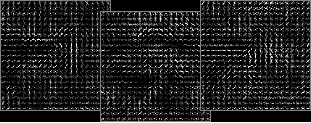
\includegraphics[width=100mm]{partbased/model/model33_555}}\\
\subfigure[K=5]{\label{fig:b}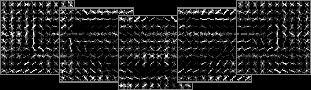
\includegraphics[width=100mm]{partbased/model/model35300_55555}} \\
\subfigure[K=7]{\label{fig:c}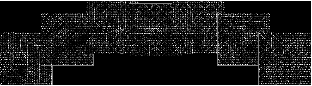
\includegraphics[width=100mm]{partbased/model/model77_5555555}} \\
\subfigure[K=9]{\label{fig:d}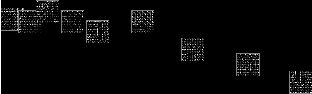
\includegraphics[width=100mm]{partbased/model/model79100_555555555}}\\
\subfigure[K=11]{\label{fig:e}
\includegraphics[width=100mm]{partbased/model/model711200_55555555555}}\\
\caption{This figure illustrate our 3, 5, 7, 9, 11 part model, demonstrate
that the additional parts up to 7 part, doesn't increase performance}
\end{adjustwidth}
\end{figure}
\todo{in table ref }
\subsubsection{Evaluation Criteria}
In this section we describe the evaluation criteria used to evaluate pose estimation.
The probability of correct pose (PCP), broadly-adopted evaluation protocol measures
the percentage of correctly localized body parts. A candidate body part is labeled as
correct if its segment endpoint lie in 50\% of the length of the ground-truth anottated
endpoints. the result of this evaluation criteria are show in the table \todo{reftable}

\subsubsection{}
\todo{organize this section}

\begin{figure}
\begin{adjustwidth}{-1in}{-1in} 
\label{fig:res537}
\centering     %%% not \center
\subfigure{\includegraphics[width=50mm]{res/ram/5_best/result0082crop}}
\subfigure{\includegraphics[width=50mm]{res/ram/5_3/result0082crop}}
\subfigure{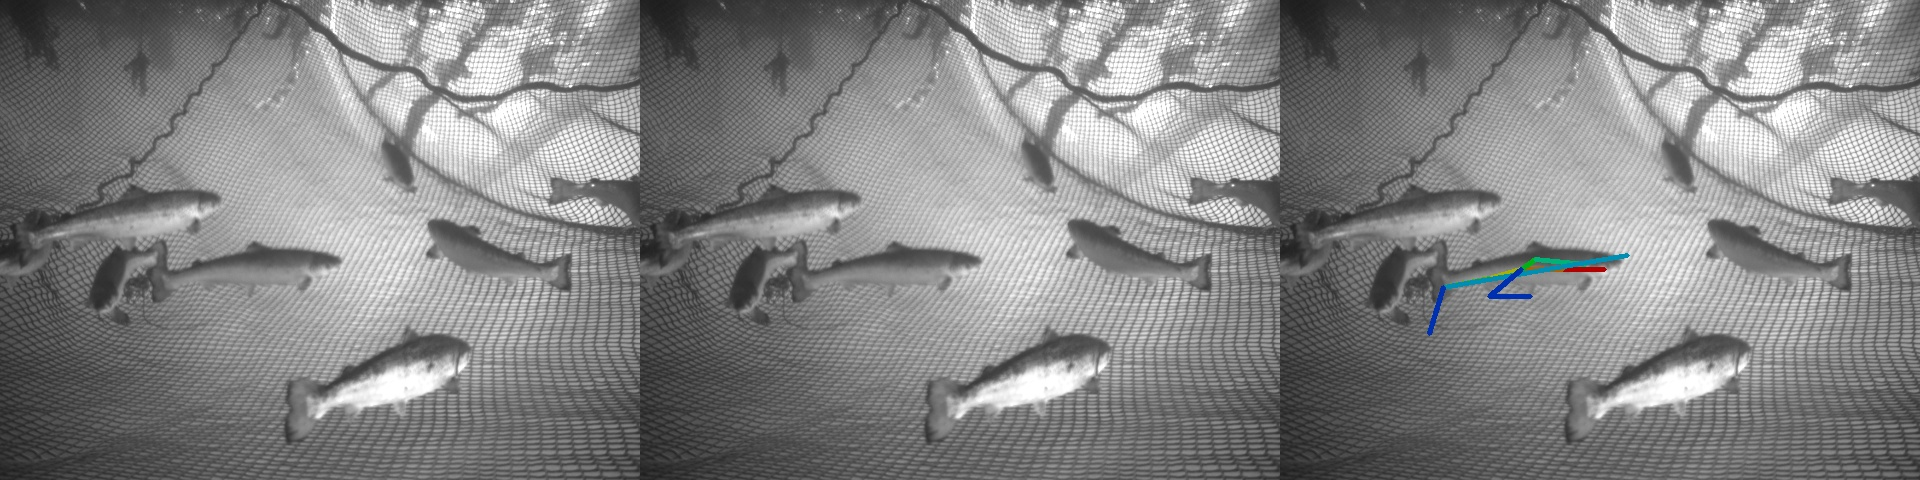
\includegraphics[width=50mm]{res/ram/5_7/result0284}}\\
\subfigure{\includegraphics[width=50mm]{res/ram/5_best/result0083crop}}
\subfigure{\includegraphics[width=50mm]{res/ram/5_3/result0083crop}}
\subfigure{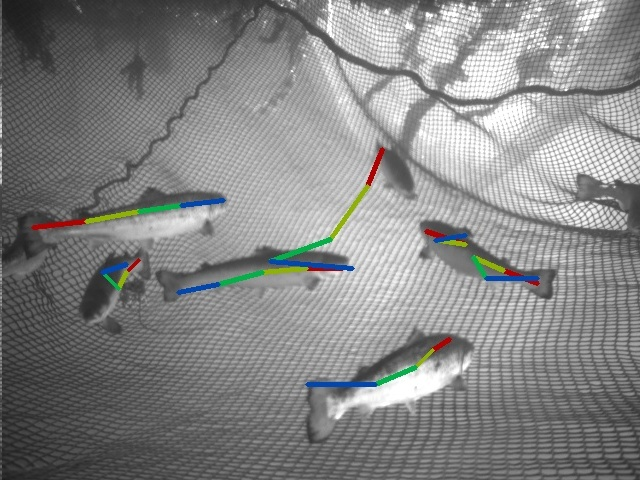
\includegraphics[width=50mm]{res/ram/5_7/result0285}}\\
\subfigure{\includegraphics[width=50mm]{res/ram/5_best/result0084crop}}
\subfigure{\includegraphics[width=50mm]{res/ram/5_3/result0084crop}}
\subfigure{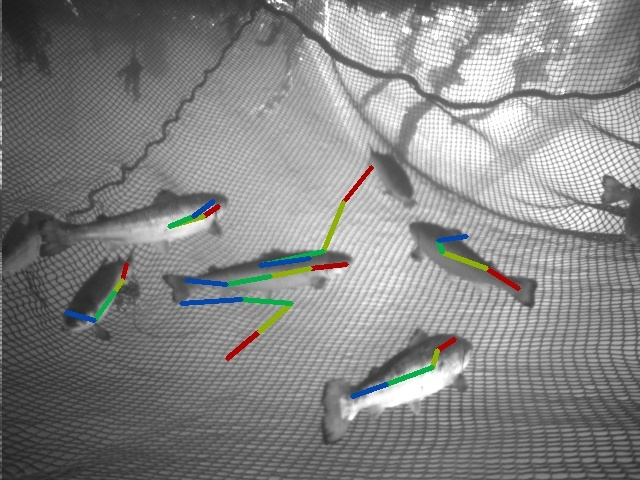
\includegraphics[width=50mm]{res/ram/5_7/result0286}}\\
\subfigure{\includegraphics[width=50mm]{res/ram/5_best/result0085crop}}
\subfigure{\includegraphics[width=50mm]{res/ram/5_3/result0085crop}}
\subfigure{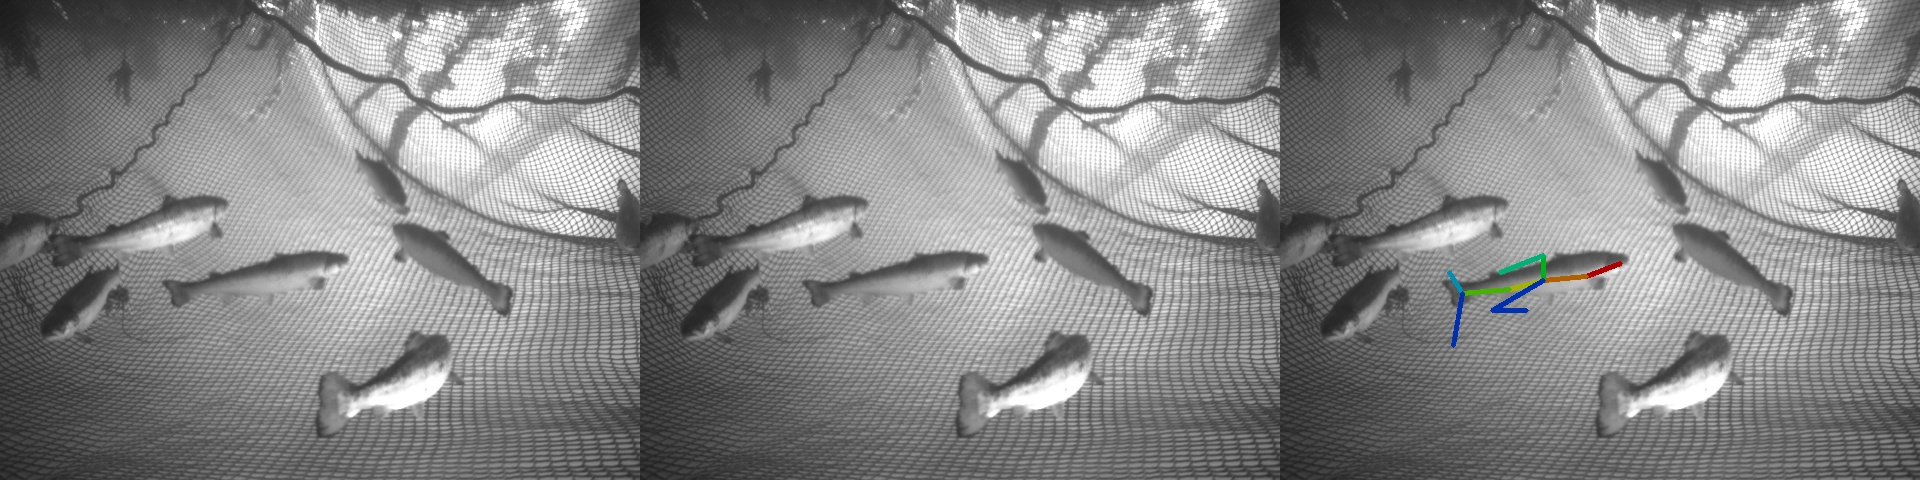
\includegraphics[width=50mm]{res/ram/5_7/result0287}}\\
\subfigure{\includegraphics[width=50mm]{res/ram/5_best/result0086crop}}
\subfigure{\includegraphics[width=50mm]{res/ram/5_3/result0086crop}}
\subfigure{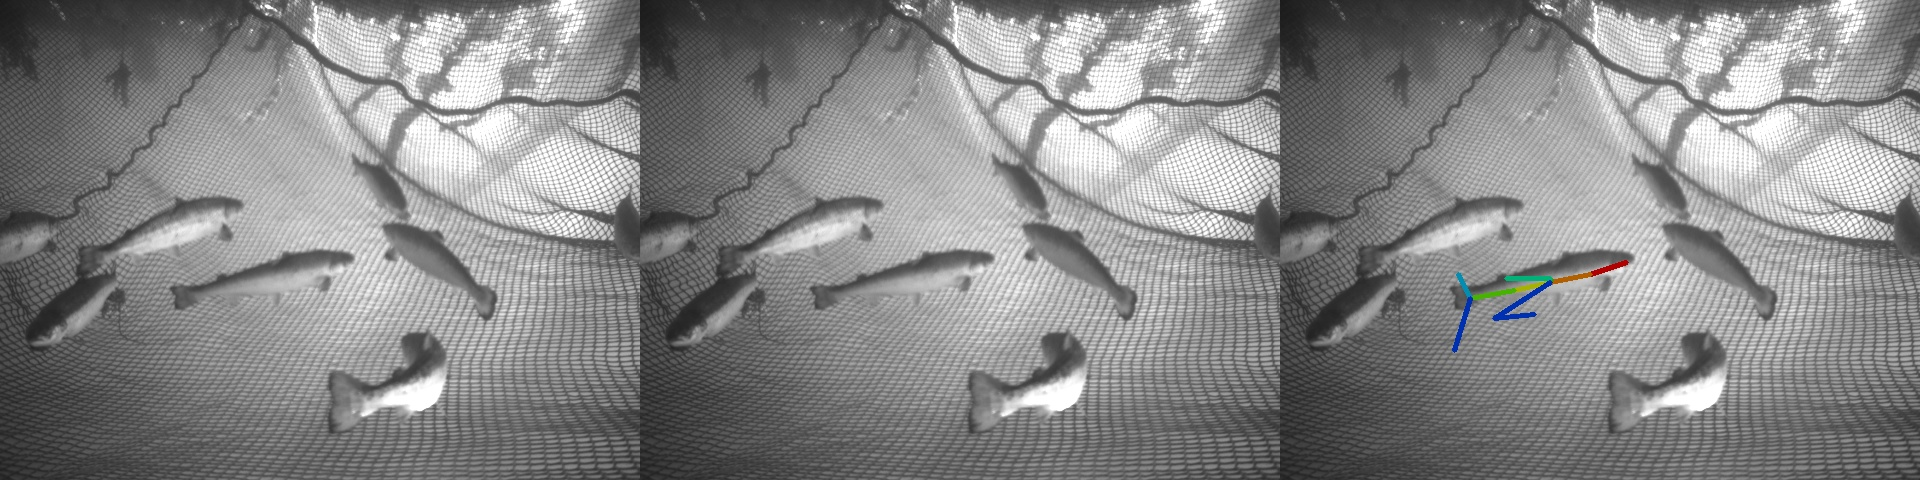
\includegraphics[width=50mm]{res/ram/5_7/result0288}}\\
% \subfigure{\includegraphics[width=50mm]{res/ram/5_best/result0087crop}}
% \subfigure{\includegraphics[width=50mm]{res/ram/5_3/result0087crop}}
% \subfigure{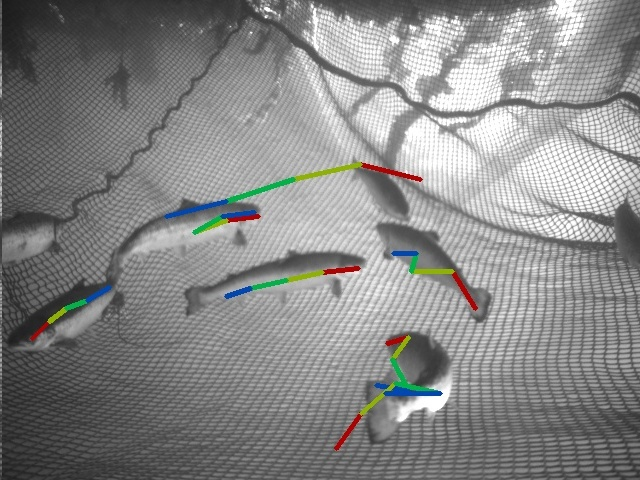
\includegraphics[width=50mm]{res/ram/5_7/result0289}}\\
\caption{5 best, 3, 7}
\end{adjustwidth}
\end{figure}


\begin{figure}
\begin{adjustwidth}{-1in}{-1in} 
\label{fig:res911}
\centering     %%% not \center
\subfigure{\includegraphics[width=50mm]{res/ram/9_11/9/result0082crop}}
\subfigure{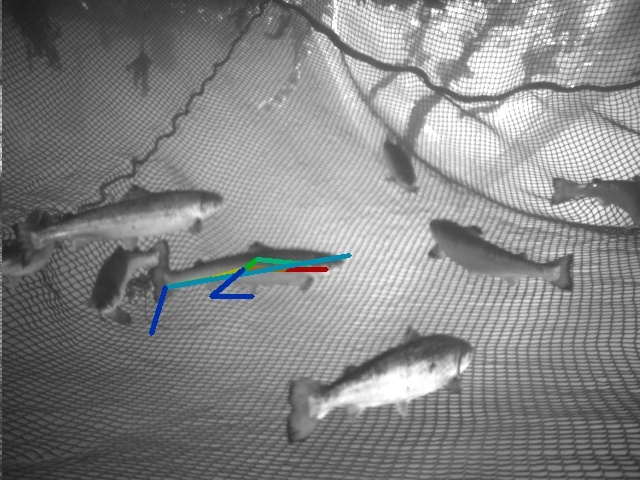
\includegraphics[width=50mm]{res/ram/9_11/11/result0284crop}}\\
\subfigure{\includegraphics[width=50mm]{res/ram/9_11/9/result0083crop}}
\subfigure{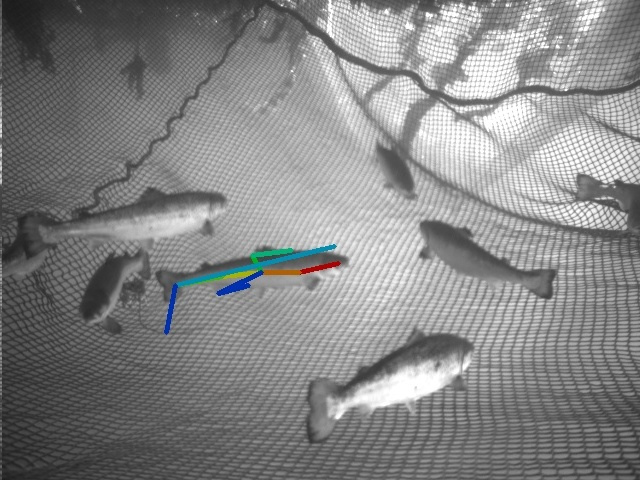
\includegraphics[width=50mm]{res/ram/9_11/11/result0285crop}}\\
\subfigure{\includegraphics[width=50mm]{res/ram/9_11/9/result0084crop}}
\subfigure{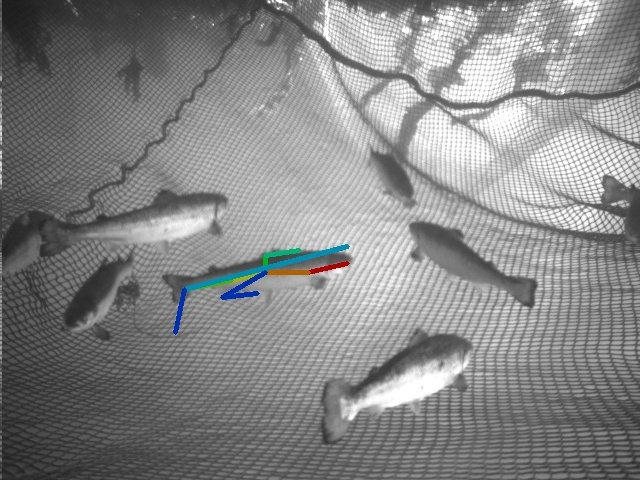
\includegraphics[width=50mm]{res/ram/9_11/11/result0286crop}}\\
\subfigure{\includegraphics[width=50mm]{res/ram/9_11/9/result0085crop}}
\subfigure{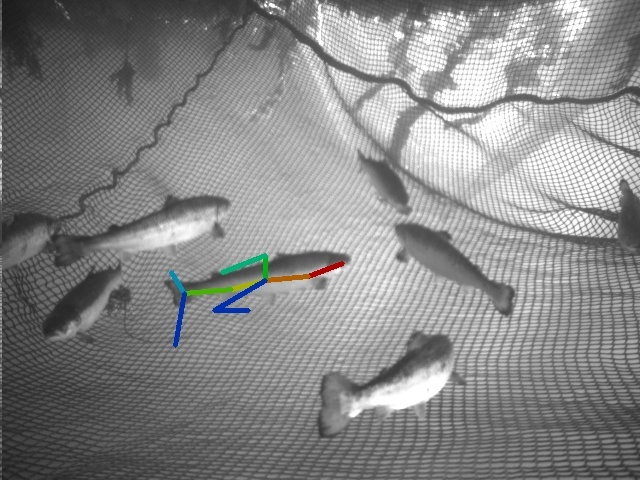
\includegraphics[width=50mm]{res/ram/9_11/11/result0287crop}}\\
\subfigure{\includegraphics[width=50mm]{res/ram/9_11/9/result0086crop}}
\subfigure{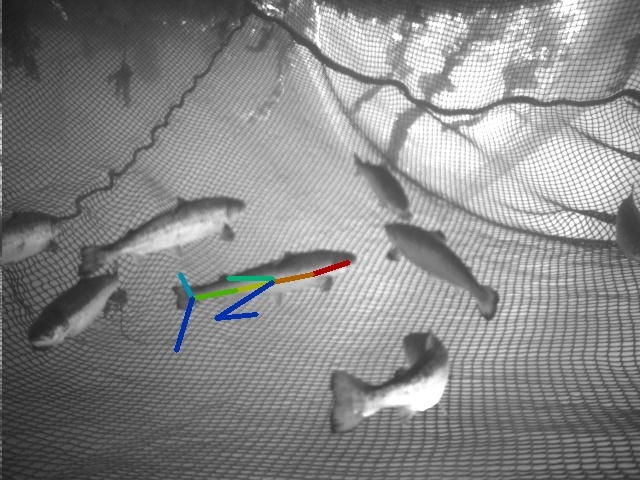
\includegraphics[width=50mm]{res/ram/9_11/11/result0288crop}}\\
% \subfigure{\includegraphics[width=50mm]{res/ram/9_11/9/result0087crop}}
% \subfigure{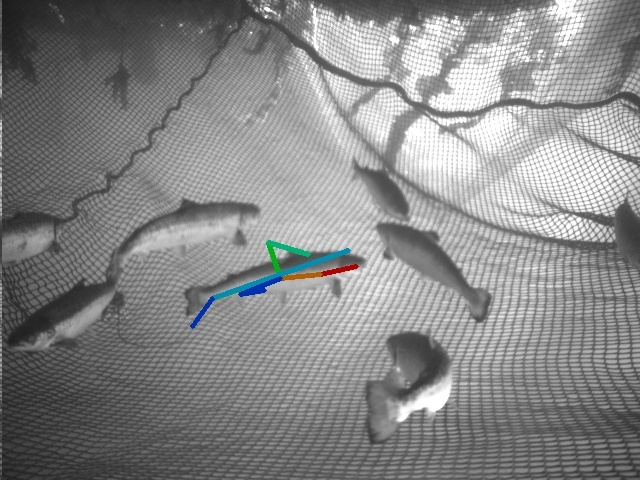
\includegraphics[width=50mm]{res/ram/9_11/11/result0289crop}}
\caption{my caption}
\end{adjustwidth}
\end{figure}

\begin{figure}
\begin{adjustwidth}{-1in}{-1in} 
\label{fig:linerambest}
\centering     %%% not \center
\subfigure{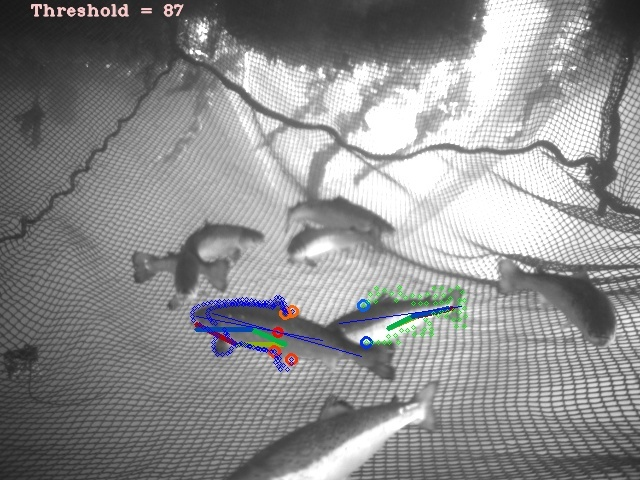
\includegraphics[width=50mm]{res/lineram/5_2best/result0011crop}}
\subfigure{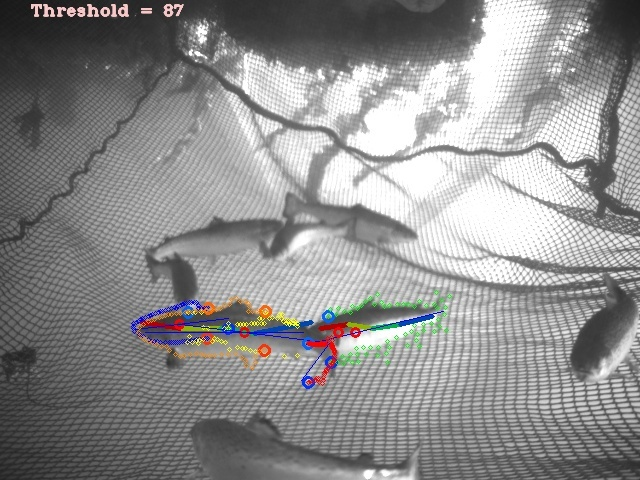
\includegraphics[width=50mm]{res/lineram/5_2best/result0013crop}}
\subfigure{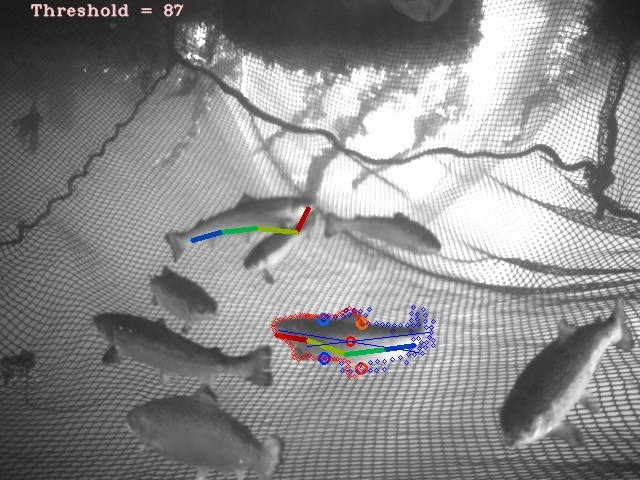
\includegraphics[width=50mm]{res/lineram/5_2best/result0016crop}}\\
\subfigure{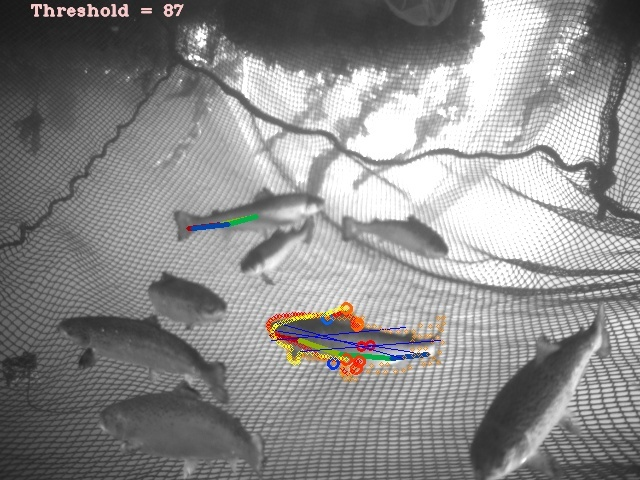
\includegraphics[width=50mm]{res/lineram/5_2best/result0017crop}}
\subfigure{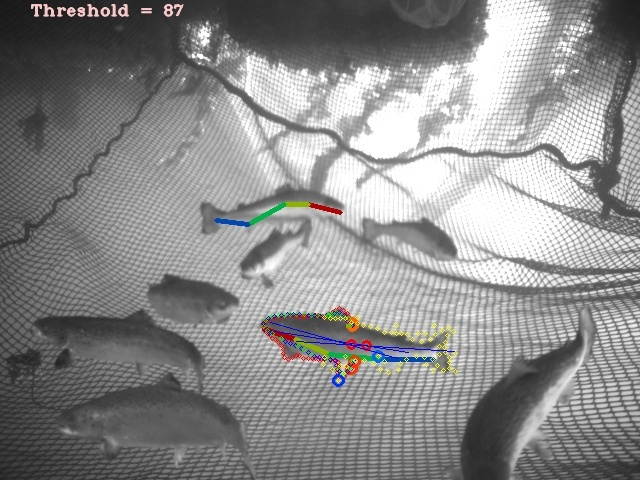
\includegraphics[width=50mm]{res/lineram/5_2best/result0018crop}}
\subfigure{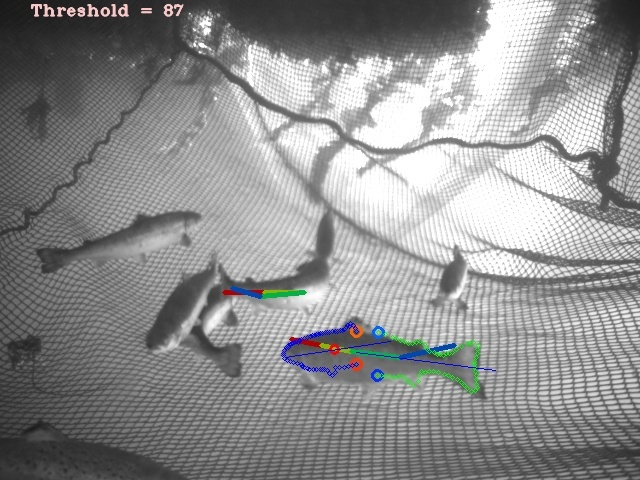
\includegraphics[width=50mm]{res/lineram/5_2best/result0034crop}}\\
\subfigure{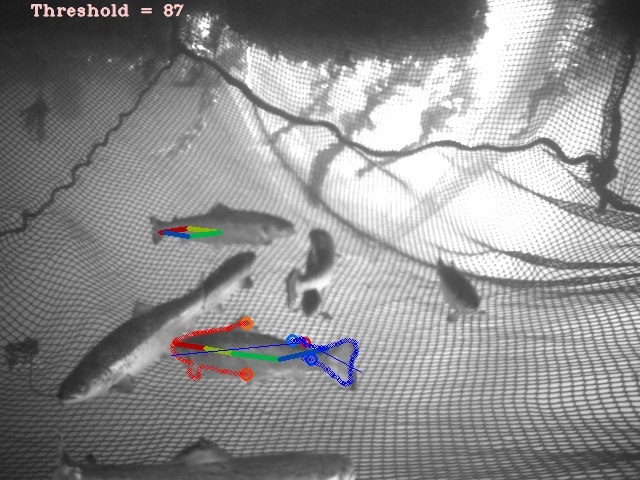
\includegraphics[width=50mm]{res/lineram/5_2best/result0040crop}}
\subfigure{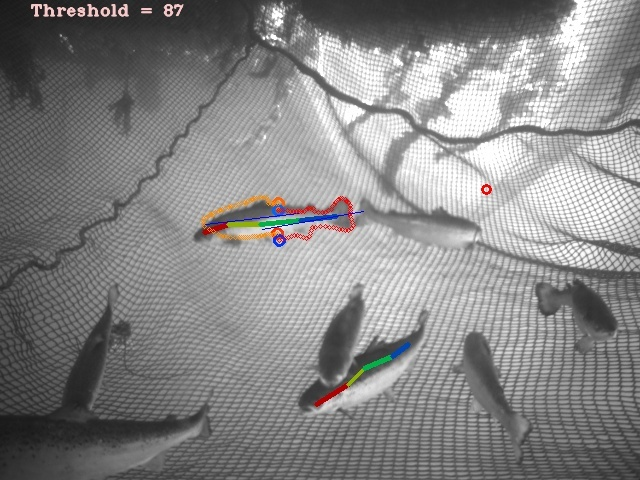
\includegraphics[width=50mm]{res/lineram/5_2best/result0056crop}}
\subfigure{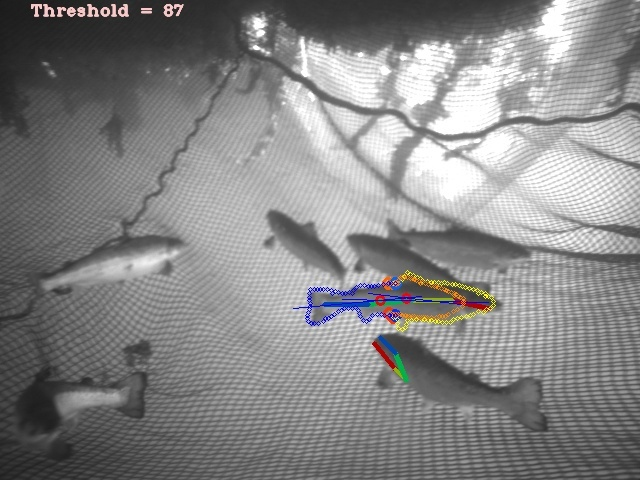
\includegraphics[width=50mm]{res/lineram/5_2best/result0099crop}}\\
\subfigure{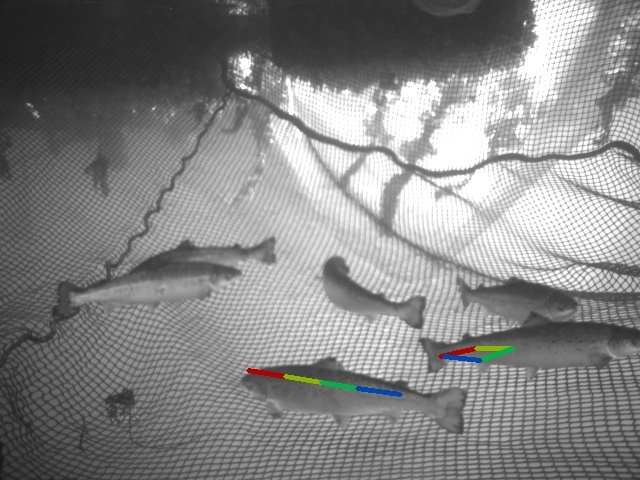
\includegraphics[width=50mm]{res/lineram/5_2best/result0107crop}}
\subfigure{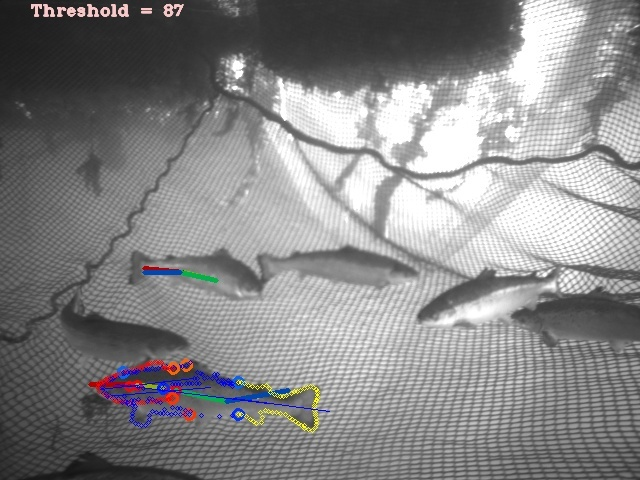
\includegraphics[width=50mm]{res/lineram/5_2best/result0116crop}}
\subfigure{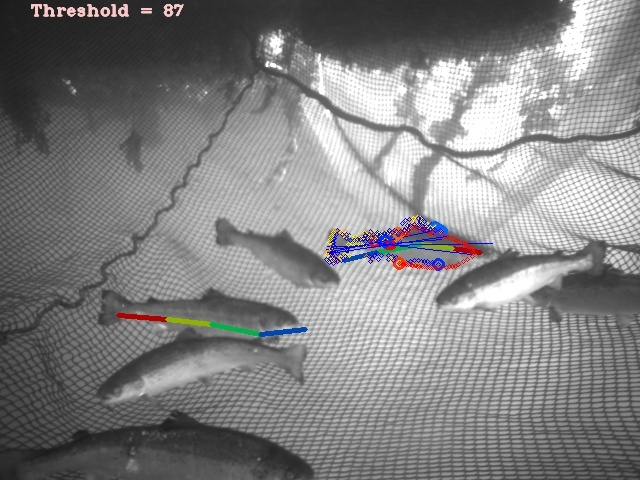
\includegraphics[width=50mm]{res/lineram/5_2best/result0119crop}}\\
\subfigure{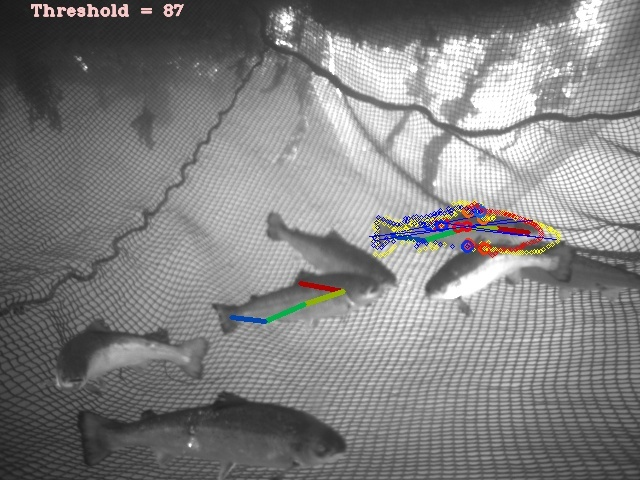
\includegraphics[width=50mm]{res/lineram/5_2best/result0124crop}}
\subfigure{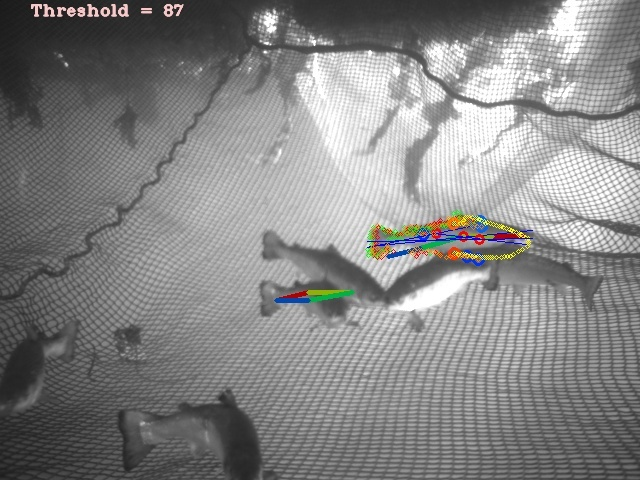
\includegraphics[width=50mm]{res/lineram/5_2best/result0127crop}}
\subfigure{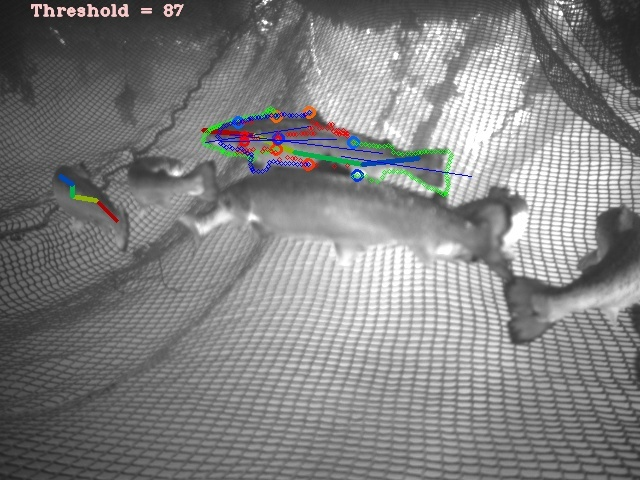
\includegraphics[width=50mm]{res/lineram/5_2best/result0165crop}}
% \subfigure{\includegraphics[width=50mm]{res/lineram/5_2best/result0261crop}}
\end{adjustwidth}
\end{figure}

\begin{table}[h]
\centering
% \cline{1-2}
\begin{tabular}{|l|l|l|ll}
Number of mixture parts & PCP  &  \\ \cline{1-2}
3     &     &          &  \\ \cline{1-2}
5     &     &          &  \\ \cline{1-2}
7     &     &          &  \\ \cline{1-2}
\end{tabular}
\caption{We evaluate various strategies for trainings parts. }
\end{table}
\todo{bring the table from the presentation}

\section{Discussion}
\todo{finish the discussion}

% \section{Next Section}
% There is no need for a latex introduction since there is plenty of literature out there.
